\chapter{Proposed Solutions}{}
\label{sec:solutions}

\section{Designing \uppercase{SnipR} operations that could be invoked directly from the search box (RQ1)}
\label{sec:rq1}
Unpacking this a bit, the key idea is to design a set of retargeting operations or commands that could be invoked from the search box, without losing any sight of the current search goal (See Chapter~\ref{chap:twist} for more details). This design should balance two inter-related principles: simplicity and flexibility. To understand what's needed to produce this type of design, this research will turn to the seminal work on sloppy command lines for the Web~\cite{Little:2007dh, Miller:2008ge} and on platform-specific linguistic command lines~\cite{Raskin:2008wb}. Similar to both types of work, the \uppercase{SnipR}'s command line will have flexible syntax requirements. This flexibility offers an important advantage. It allows queries and retargeting requests to be intermixed---or used separately. The focus of these commands---and language---will be twofold. First, to interact with search result. Second, to perform code modifications on retrieved code examples. For simplicity, SNIPR will provide most of the mechanisms for expression and control of changes that could be made to modules (methods that implement an API). This involves discovering the fundamental concepts of retargeting modules, to extract them from their various reincarnations, and to present them in a pure and distilled form. This form will be inspired by the syntax of the Io programming language\footnote{\url{http://iolanguage.org/}}. For flexibility, a simple language for combining, and executing code retargeting commands will be developed. This language's goal is to extend \uppercase{SnipR}'s available functionality. 
% Previous work in command lines for code modifications exist and could be usually seen implemented as plugins in mainstream IDEs, such as Eclipse\footnote{\url{http://www.eclipse.org}} and IntelliJ IDEA\footnote{\url{http://www.jetbrains.com}}. In contrast, with \uppercase{SnipR}, developers will continue to use their Web browser to do these code modifications. 

\fancybreak{\pfbreakdisplay}

\section{Performing Code Retargeting (RQ2, RQ3, and RQ4)}
\label{sec:restqs}
Code modification---to make code more suited---or retargeting is an operation that can work on a single search result or an entire result set. Therefore, this operation requires that those cases where code mappings can be learned and/or applied are carefully identified. This will prevent any unnecessary work from happening as matched code examples are being returned by the query engine. This requirement will be addressed by developing a set of reliable and cache conscious \uppercase{SnipR} algorithms (RQ2). They should be reliable in the sense of consistently learning code mappings from example code. They should be cache conscious in the sense of exploiting recently read example code if this code must be read again in the future. The output of these algorithms are code mappings that are applied by the query engine when retargeting is needed (See Chapter~\ref{chap:algorithms} for more details). In order for the query engine to do that, a set of code retargeting operators well-suited for manipulating example code within query processing must be created (RQ2). These operators should be reliable in the sense of applying learned mappings. Moreover, they should be implemented within the querying processing step of a working code search engine (RQ3). 

As for the rules that would guide the retargeting of found code, this research will turn to developing a prototype, which will represent code searching as a short cycle of alternating query, retarget (or the intermixing thereof), and screen phases. By leveraging the experience gained with this prototype, a model for retargeting found code will be developed. This model will allow a formal reasoning about any experimentation in the \uppercase{SnipR}'s design space, and a path to an efficient implementation of \uppercase{SnipR}. 

In retrospect, if the developer retargets code in advance, then the evaluation results are available immediately, which saves valuable time searching for appropriate example code (See Figure~\ref{fig:retargeting}). By saving this time, the developers will get the work done more quickly (RQ4). This will be possible only if \uppercase{SnipR}'s retargeting operations are efficient, which will be demonstrated by answering RQ2. 

% Previous work in adapting code to alternate contexts and/or to new APIs exist. Such work has helped developers with many development tasks, such as adapting example code to new contexts~\cite{Wightman:2012gc} or to new APIs~\cite{Nita:2010en}. This also includes resolving many simple coding errors quickly\footnote{{Quick Fix Scout: \url{https://code.google.com/p/quick-fix-scout/}}, {EUKLAS: \url{http://www.cs.cmu.edu/~euklas}}}, or suggesting ways for correcting compiler and runtime errors~\cite{Hartmann:2010hx}. Unlike \uppercase{SnipR}, any interaction for finding and changing any example code or suggesting solutions to a problem in the developer's code is directly done in the IDE.

\fancybreak{\pfbreakdisplay}

\section{Evaluation}
\label{sec:evaluate}

The evaluation methodology to be followed is to validate the \uppercase{SnipR} approach and results through user and lab studies. The tests will be run on \uppercase{SnipR} prototypes in a working code search system, such as Sourcerer\cite{Bajracharya:2006vn} or another Internet-scale code search engine. The user studies will involve a list of subjects, solicited from a public mailing list at a college campus. The subjects will also be experienced Web users, have some programming experience, and could type reasonably well. The use and test of the \uppercase{SnipR} prototype will be done on the basis of a programming problem to be solved; aiming to answer the research questions listed in Section~\ref{sec:questions}. For instance,

\begin{itemize}  
\item A user study will be performed to test for the flexibility and simplicity of the developed command-line language (called Twist)---see Chapter~\ref{chap:twist} for more details. The test attempts to determine how intuitive this language is for end-users. The test is also used to determine how this language might be used in daily development activities and to evaluate some of the decisions made on the design of the language's ``intuitively readable commands.'' Each subject will sit at a computer loaded with a \uppercase{SnipR}--aware code search system. Each subject will be directed to a website to receive instructions on how to start using \uppercase{SnipR}. The instructions will indicate that each subject should only use the search box to do any of the assigned tasks. The instructions will also state a programming problem to be solved; i.e., changing a sentiment analysis tool (that uses Twitter API) to use the Facebook API. After the subjects have completed the tasks, a survey will be given to the subjects to ask them about their experience with \uppercase{SnipR}. The data gathered from this test and survey will shed light on ease of use, and flexibility of the created commands (RQ1).

\item In addition to creating and using a set of microbenchmarks, the same user study is also used to provide a feel for the speed and accuracy of the  \uppercase{SnipR} algorithms. Inputs from the user study will be used to derive an average processing time---in terms of learning and applying code mappings from/to example code. It is expected that the processing time varies for input sizes of different lengths. From this, one could guess that the average-case running time is polynomial, but that it is reasonable for relatively small source code (e.g., less than 40 lines of code~\cite{Brandt:2009ew}), such is the case of example code (RQ2). 

\item To evaluate the effectiveness of the learning algorithm, a hold-out test will be run. A set of mappings extracted from a collected corpus will be used as training data, and another different set of mappings---randomly chosen---as a test data. The generalized perceptron (described in Chapter~\ref{chap:algorithms}) will be run for a given number of iterations. The output of this will be a cost model, which will be used to predict mapping-based program transformations.

\item A lab study will be conducted to gauge the goodness of where in the query processing step the retargeting operators should be implemented. For this lab study three versions of a working code search system will be released. The first version, \uppercase{SnipR}--A, will have these operators implemented within the interpreter of the command line language. The second version, \uppercase{SnipR}--B, will have these operators nested inside the query engine's retrieval process (see Figure~\ref{fig:irarchitecture}). The third version, \uppercase{SnipR}--C, will have these operators implemented as part of the ranking process of the query engine (see Figure~\ref{fig:irarchitecture}). This lab attempts to estimate how responsive these operators are when facing many different types of workloads---i.e., queries or commands issued by a user. This lab is also used to provide a feel for the scalability of these operators (which is expected to be high). The data gathered from this lab will shed light on where \uppercase{SnipR} belongs within the query processing step of any modern code search engine (RQ3). 

\begin{figure}[!ht]
    \centering
    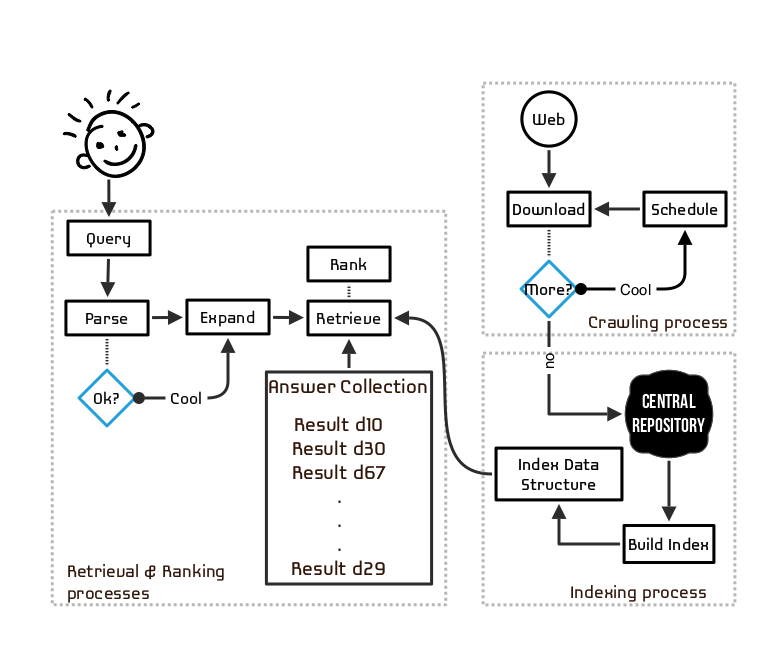
\includegraphics[width=\textwidth]{images/csarchitecture}
    \caption{High level architecture of a code search engine.}
    \label{fig:irarchitecture}
\end{figure}
\pagebreak

\item In addition to the above user and lab studies, a new user study will be conducted comparing \uppercase{SnipR} to a general Web code search engine (e.g., Koders) and an example-centric programming tool that enhances a search interface (e.g., SnipMatch or Blueprint). This study attempts to examine how quickly developers perform a more complete code search task (with or without \uppercase{SnipR}), the quality of the solutions obtained, and the number of queries issued. This study will be based on the subjects trying to solve a programming problem by doing code search. The subjects will be asked not to write any code from scratch, but to instead find example code that best matches the problem at hand. A Latin Square design will be used to control the order in which the search interfaces are presented to subjects at the beginning of the experiment. The data gathered from this study will be used to gauge how efficient the \uppercase{SnipR} approach is in comparison to general and/or code-centric search engines (RQ4).     
\end{itemize}

\fancybreak{\pfbreakdisplay}

\section{Timeline}
\label{sec:workplan}

I expect to take approximately two years to finish from this point. I am 
focusing on the opportunities and challenges outlined in this document. 
Meanwhile, I continue to refine my thesis proposal, and get feedback from other 
researchers. 

\begin{itemize}
\item Winter 2013 - Fall 2014. The first year will focus on stretching 
    \uppercase{SnipR} into an efficient practice.
    \subitem Flesh out command line language (refining and describing all 
    commands in detail).
    \subitem Flesh out system architecture (refining and describing all 
    components in detail).
    \subitem Flesh out \uppercase{SnipR}, the learning algorithm for mapping-based transformations,  
	 the algorithm for applying these mappings, and code retargeting operators.  
    \subitem Write up several position papers on \uppercase{SnipR} using the above discoveries.
    \subitem Implement and integrate the system.
\item Winter 2014 - Fall 2015. The second year will focus on architectural 
    experimentation, evolving the system, and generalizing this work's 
    contributions; including the writing of my dissertation.
    \subitem Write up the initial results product of system integration and 
    architecture.
    \subitem Carry out user experiments; including the evaluation of all \uppercase{SnipR}'s algorithms.
    \subitem Perform a final literature review. 
    \subitem Produce a detailed thesis outline conditioned on experimental 
    results.
    \subitem Finish writing and defend.
\end{itemize}
